\documentclass[12pt, twoside, a4paper]{article}

\usepackage[utf8]{inputenc}
\usepackage[english]{babel}
\usepackage{csquotes}

\usepackage[margin=1in,left=1.5in,includefoot, a4paper]{geometry}

\usepackage{pythonhighlight}
\usepackage{listings}

% Python style for highlighting
\newcommand\pythonstyle{\lstset{
language=Python,
basicstyle=\ttm,
otherkeywords={self},             % Add keywords here
keywordstyle=\ttb\color{deepblue},
emph={MyClass,__init__},          % Custom highlighting
emphstyle=\ttb\color{deepred},    % Custom highlighting style
stringstyle=\color{deepgreen},
frame=tb,                         % Any extra options here
showstringspaces=false            % 
}}

% Python environment
\lstnewenvironment{ipython}[1][]
{
\pythonstyle
\lstset{#1}
}
{}

% Header and Footer
\usepackage{fancyhdr}
\pagestyle{fancy}
\fancyfoot{}
\fancyhead{}
\renewcommand{\headrulewidth}{0pt}
\fancyfoot[LE]{\thepage}
\fancyfoot[RO]{\thepage}
%\fancyfoot[LE,RO]{\thepage}

% Custom colors
\usepackage{color}
\definecolor{deepblue}{rgb}{0,0,0.5}
\definecolor{deepred}{rgb}{0.6,0,0}
\definecolor{deepgreen}{rgb}{0,0.5,0}

\usepackage{graphicx}
\usepackage{subfig}
\usepackage{float}

\usepackage{biblatex}

\addbibresource{references.bib}

\begin{document}

\begin{titlepage}
    \begin{center}
        \vspace*{.06\textheight}{\scshape\LARGE Birkbeck, University of London\par}\vspace{1.5cm} % University name
        \rule[0.5ex]{\linewidth}{2pt}\vspace*{-\baselineskip}\vspace*{3.2pt}
        \rule[0.5ex]{\linewidth}{1pt}\\[\baselineskip]
        \huge{\bfseries Pneumonia Detection from Chest X-Ray Images\\ Draft}\\[4mm]
        \rule[0.5ex]{\linewidth}{1pt}\vspace*{-\baselineskip}\vspace{3.2pt}
        \rule[0.5ex]{\linewidth}{2pt}\\
        [1.5cm]


        \begin{minipage}[t]{0.4\textwidth}
        \begin{flushleft} \large
        \emph{Author:}\\
        {Baran Buluttekin} % Author name - remove the \href bracket to remove the link
        \end{flushleft}
        \end{minipage}
        \begin{minipage}[t]{0.4\textwidth}
        \begin{flushright} \large
        \emph{Supervisor:} \\
        {Dr. George Magoulas} % Supervisor name - remove the \href bracket to remove the link  
        \end{flushright}
        \end{minipage}\\
        [3cm]

            \vfill

            \large \textit{A thesis submitted in fulfillment of the requirements\\ for the degree of MSc Data Science}\\[0.3cm] % University requirement text
            \textit{in the}\\[0.4cm]
            Department of Computer Science\\[2cm] % Research group name and department name
 
            \vfill

            {\large \today}\\[4cm] % Date
            %\includegraphics{Logo} % University/department logo - uncomment to place it
 
            \vfill
    \end{center}
\end{titlepage}    
\thispagestyle{empty}
\cleardoublepage

\pagenumbering{roman}
\section*{Abstract}
\addcontentsline{toc}{section}{Abstract}
This is placeholder text. To add more information type it after this line.\\
\clearpage


\section*{Declaration}
\addcontentsline{toc}{section}{Declaration}
I hearby declare this file a text.

\begin{python}
    import pymongo as pm
    import json
    # line comment
    with open("DSTA/Lab/mongo.json") as f:
    url = json.load(f)
    """ Comment 1"""
    "Comment 2"

    c = pm.MongoClient(url["url"])

    def Myfunc(x):
        print(x)

    print(c.admin)
\end{python}
and text goes on.\\
\clearpage

\tableofcontents
\thispagestyle{empty}
\cleardoublepage
    

\pagenumbering{arabic}
\setcounter{page}{1}


\section{Introduction}

Pneumonia is swelling (inflammation) of the tissue in one or both lungs. It is usually formed at the end of breathing tubes of the lungs and cause these tubes to inflame and fill up with fluid. In the UK, pneumonia effects around 8 in 1000 adults each year \cite{nhs}. Global economic cost of pneumonia has estimated at \$17 billion annually \cite{cost}. Currently detecting pneumonia cases heavily relies on chest X-ray image examination which requires expert radiologists to diagnose. Building intelligent system to diagnose the pneumonia can help  health care services to increase efficiency and reduce costs and could help increase early diagnoses in countries with inadequate access to health care.

\subsection{Related Work}

There are number of research has been published about lung diseases related detection. Most prevalent ones are the CheXNet \cite{CheXNetRP} and ChestX-ray8 \cite{ChestX-ray8}, both of these research carried out by training on same dataset ChestX-ray8 \cite{ChestX-ray8}. ChestX-ray8 comprises of approximately 100,000 frontal view chest X-ray images labelled by extracting information from the accompanied radiologists notes with using variety of different NLP (Natural language processing) techniques from the openi\cite{openi} database. ChestX-ray8 authored by researchers from National Institute of Health (NIH) and published at 2018.
Most profound effect of this paper is the creation of the ChestX-ray8 dataset which has become one of the widely used dataset in computer vision research related to lung diseases. More detailed information about the dataset can be found in dataset section of this proposal. 

CheXNet is another related article authored by researchers from Stanford University ML group. Prediction of lung diseases achieved by 121 layer convolutional neural network and designed to predict 14 pathologies in the ChestX-ray8 dataset. One of the major importance of this paper is the setting the setting benchmark for human level detection for chest X-ray images. One of the most fundamental difference of the X-ray related disease prediction is the definition of human level accuracy. Due to the nature of required expertise in X-ray images leaves general public out of the scope when it comes to human level performance of these pathologies. Anyone who have not been trained in radiology will not be able to detect any lung diseases in the Chest X-ray images. For example the image below is sample of two chest X-ray images almost indistinguishable to general audience.

\begin{figure}[H]%
    \centering
    \subfloat{{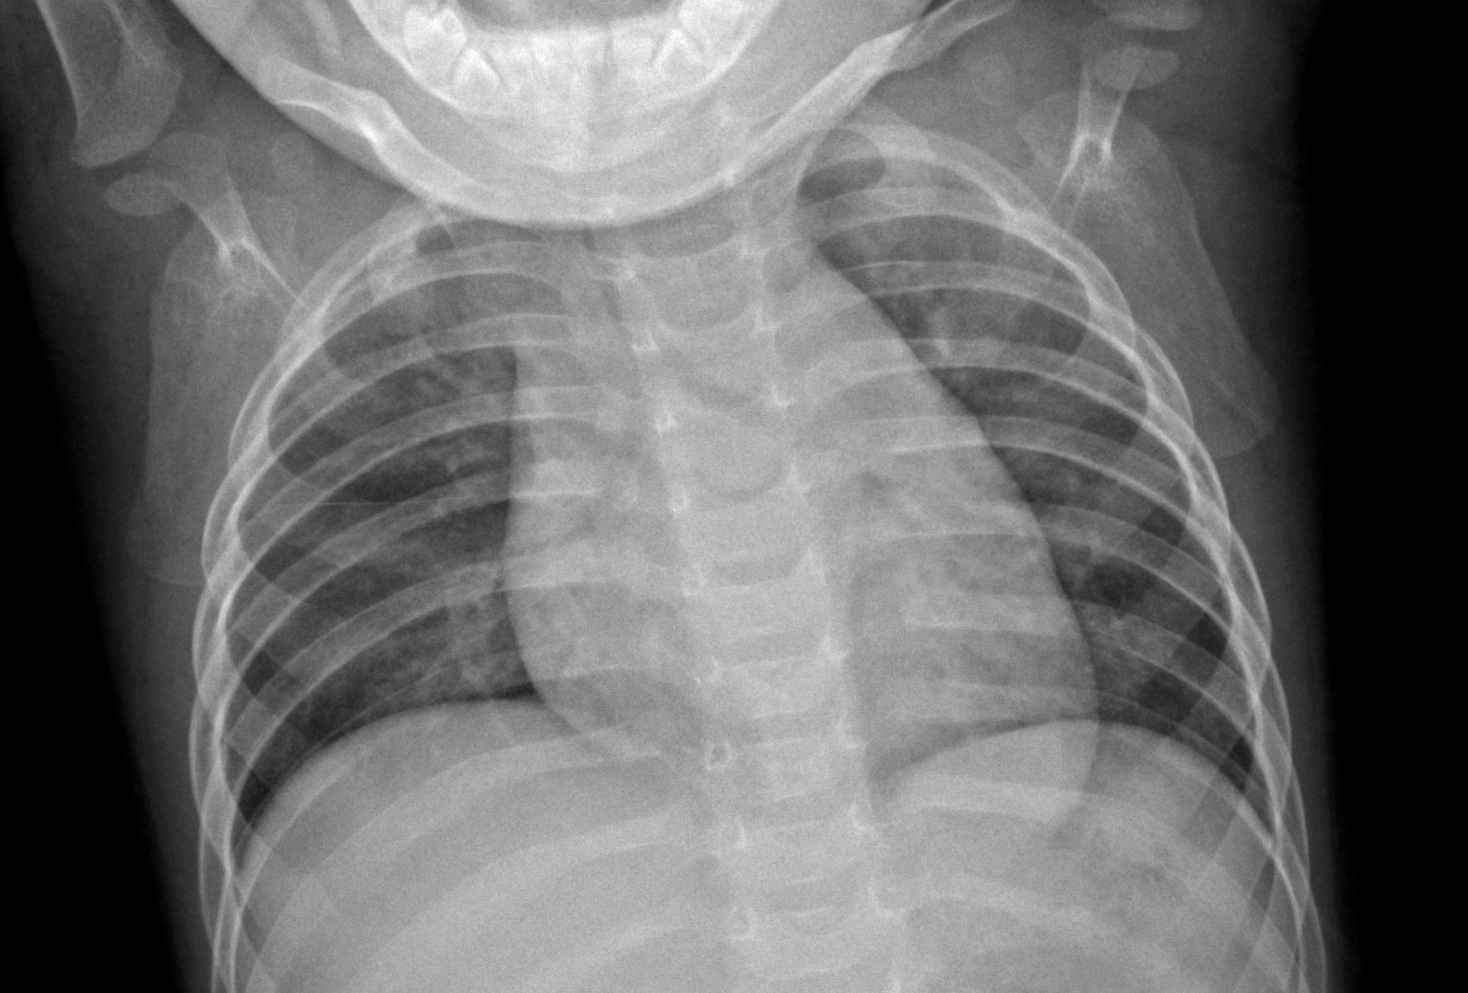
\includegraphics[width=.4\textwidth]{img/chest_xray_train_NORMAL_IM-0133-0001.jpeg} }}%
    \qquad
    \subfloat{{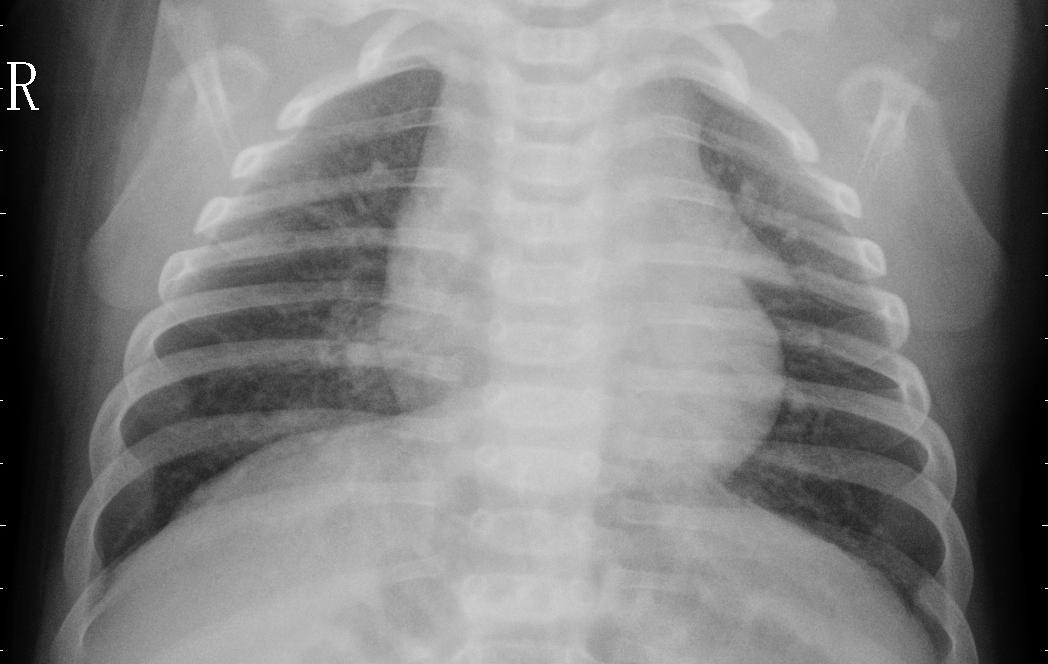
\includegraphics[width=.4\textwidth]{img/chest_xray_train_PNEUMONIA_person1007_virus_1690.jpeg} }}%
    \caption{Two sample X-ray Chest images.}%
    \label{fig:sample}%
\end{figure}
Given this challenge authors of the CheXNet conduct a test to establish benchmark for radiologists. They have collected 420 frontal chest X-rays and asked practicing radiologists in Stanford University to label them for all 14 pathologies. Radiologists selected with different range of experience, and had 4, 7, 25 and 28 years of experience. X-ray images presented to radiologists without any patient information or any symptoms experienced by patients and their diagnoses predictions measured based on underlying state of the X-ray patients. Fallowing is the table showing the summary statistic of this test for the 4 radiologists participated to test on F1 score, which is harmonic average of precision and recall.\cite{CheXNetRP}:
\begin{table}[h!]
    \centering
     \begin{tabular}{l r} 
     \hline
      & F1 Score (95\% CI) \\ [0.5ex] 
     \hline
     Radiologists 1 & 0.383 (0.309, 0.453) \\ 
     Radiologists 2 & 0.356 (0.282, 0.428) \\
     Radiologists 2 & 0.365 (0.291, 0.435) \\
     Radiologists 4 & 0.442 (0.390, 0.492) \\
     \hline
     Radiologists Avg & 0.387 (0.330, 0.442) \\ [1ex] 
     \hline
     \end{tabular}
     \caption{Radiologist prediction performances from CheXNet.}
     \label{table:radiologist}
\end{table}

Importance of this test is that it gives us a rough estimate for human level accuracy benchmark to assess the model performance for new detection models.


\clearpage
\section{Dataset}
Choosing and processing dataset have a crucial importance on success of the any machine learning task. There are several dataset available online that relate to chest X-Ray images. Given the large number of choices for selecting the dataset there are few criteria important to check while deciding the final dataset.

\subsection{General Guidelines While Deciding on the Dataset}
In this section I have highlighted my reasons for deciding on the dataset of choice for this research project. Main points for decision are:
\begin{enumerate}
    \item \textbf{Reproducibility: }Dataset of choice must allow reader to reproduce the work in order to assess all the points discussed in the report. That would require dataset to be public.
    \item \textbf{Labelled: }Dataset must contain labels of patients state. Such as being diagnosed with pneumonia or not.
    \item \textbf{License: }Dataset should have a license that permits research.
\end{enumerate}
I will be evaluating dataset available while considering general guidelines outlined above.

\subsection{OpenI Database}

OpenI\cite{openi} is a database that is service of National Library of Medicine. It enables search for medical images, graphs and charts through text as well as image query. As of writing of this proposal it has over 3.7 million images, and 3,955 radiology reports. It is the main source for ChestX-ray8 dataset mentioned previously in Related Work section. Despite the fact it contains very large data for chest X-rays, this source is not suitable for this project due to the fact that images does not includes labels for the patients state (e.g., Pneumonia or normal). Chest X-ray data in this database is the image accompanied by radiologist report which is advisory to doctors.

\subsection{ChestX-ray8}
This dataset created part of the ChestX-ray8\cite{ChestX-ray8} paper. Original source of this dataset is OpenI\cite{openi} medical database as mentioned in previous subsection.

\subsection{Cell Press Research}
\clearpage

\section{Computer Vision}
\subsection{Convolutional Neural Networks (CNN's)}
\subsection{Prominent Computer Vision Architectures}
\subsection{AlexNet}
\subsection{VGGNet}
\subsection{Inception}
\subsection{YOLO}
\clearpage

\section{Project Aims and Objectives}
\clearpage

\section{Tools and Techniques}
\clearpage

\section{Project Plan}
Early draft to be completed later.
\clearpage

\printbibliography
\addcontentsline{toc}{section}{References}

\end{document}